\documentclass[conference,onecolumn]{IEEEtran}
\usepackage{graphicx}
\usepackage{amsmath}

\setlength{\parskip}{0.5em}
% \setlength{\parindent}{0pt}


\begin{document}

\title{Landslide Susceptibility Mapping with GIS-Based Conditional Adversarial Networks}

\author{
\IEEEauthorblockN{Mohamed Mafaz}
\IEEEauthorblockA{
IIT Madras\\
Chennai, India\\
am25m009@smail.iitm.ac.in}
\and

\IEEEauthorblockN{Akul Pradeep}
\IEEEauthorblockA{
BSACIST\\
Chennai, India\\
akulpra12@gmail.com}
\and

\IEEEauthorblockN{Dr.~Aisha~Banu~W}
\IEEEauthorblockA{
BSACIST\\
Chennai, India\\
hodcse@crescent.education}
\and

\IEEEauthorblockN{Syed~Mohammad~Shoaib}
\IEEEauthorblockA{
KL University\\
Vijayawada, India\\
2501050041@kluniversity.in}
}

\maketitle

\maketitle

\begin{abstract}
A landslide is the movement of a mass of rock, debris, or earth down a slope. Landslides are a type of “mass wasting,”
which denotes down-slope movement of soil and rock under gravity [1]. in India, about 0.42 million sq. km or 12.6% of land area,
excluding snow covered area, is prone to landslide hazard [2]. Landslide susceptibility mapping is the process of identifying areas
prone to landslides amid natural changes to that of the geology, tropical factors, environmental factors and many more. In process
of mapping these regions and classifying them into different categories of threat level, it help in early detection and avoidance. By
using EOBrowser [3] to quickly view and analyze different algorithms, this paper shows promise of easier and accurate landslide
mapping. After Mapping of existing landslide cases, those cases where taken in during Data Collection process further fed into
Conditional Adversarial Network for prediction of LSM before it happens. During data collection process various factors where
cross referenced and: NDVI, dNDVI, Slope, Elevation, NDWI, Barren soil index where ranked as the most important one of them
all.
\begin{figure}[htbp]
    \centering
    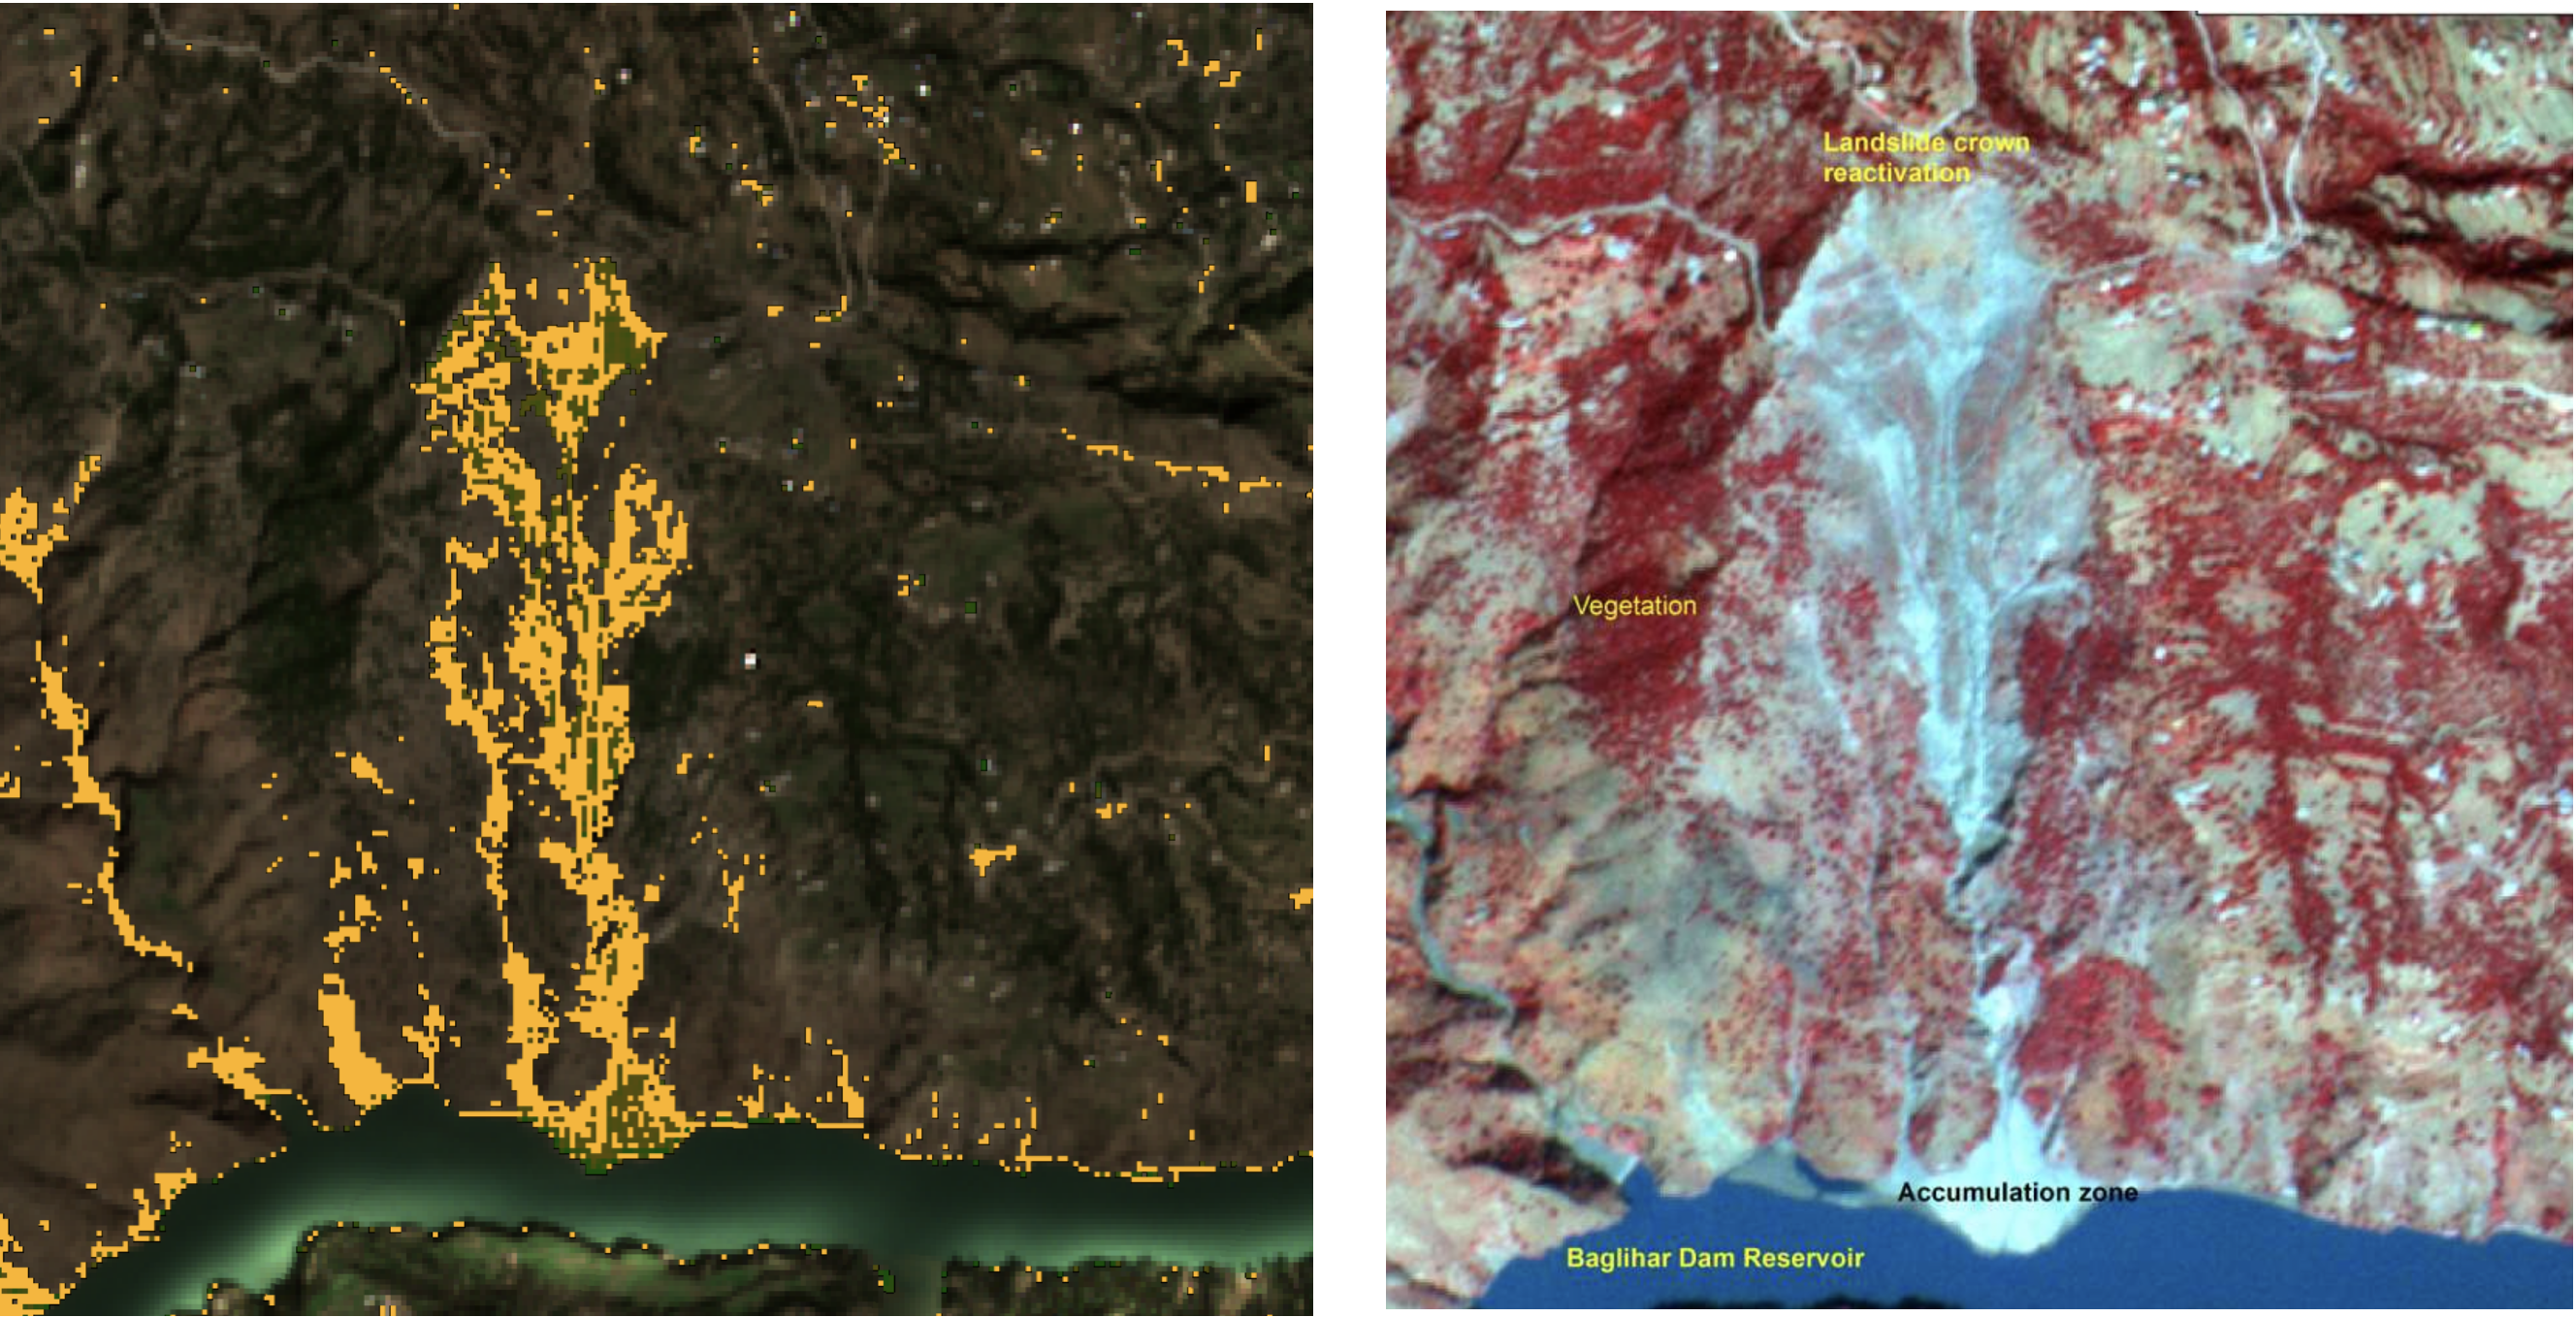
\includegraphics[width=0.6\linewidth]{images/1_abstract.png}
    \caption{Our algorithm vs Landslide Atlas of India [1]}
    \label{fig:1_abstract}
\end{figure}

\end{abstract}

\begin{IEEEkeywords}
Landslide susceptibility mapping, EOBrowser, NDVI, dNDVI, Slope, Elevation, NDWI, Barren soil index.
\end{IEEEkeywords}

\section{Research Area}
Since Landslide susceptibility mapping is one of the important junctures of geospatial analysis, remote sensing, and machine learning, which focuses on the prediction of zones that are susceptible to slope failure. In India alone, it is revealed that about 0.42 million square kilometers of area or 12.6 percent of the land area is prone to landslides; therefore, accurate prediction of landslides is imperative for preparing for such natural calamities. This research area explores the application of GIS, satellite remote sensing, and sophisticated computational techniques for terrain stability analysis.​​

\subsection{Traditional Ways of Solving the Problem}
Traditional techniques for susceptibility zonation of landslides make use of statistics, as well as models developed by experts that identify the factors that trigger landslides, including slope, elevation, geology, distance from faults, rainfall, and land use. Such models are often capable of producing a susceptibility map that divides an area into zones of low, moderate, or high susceptibility. But these models tend to encounter shortcomings with respect to scalability or real-time processing.​​

\subsection{Deep Learning / Generative Models}
Recently, the trends in the field have moved towards machine learning-based or deep learning-based models for learning complex spatial patterns for geospatial data with high dimensionality. One such recent advancement in deep learning models is the application of Generative Adversarial Networks (GANs), especially Conditional GANs (cGANs), for image-to-image translation tasks in geospatial applications. Such techniques have the capability of learning the complex dependencies between multiple indicators of the environment and produce accurate susceptibility maps with the help of various inputmodalities such as vegetation indices, water content, terrain, and soil exposures. This work rectifies the drawbacks of the existing methods by learning multiple indicators together for accurate predictions at high resolution for various geospatial applications

\section{Literature Survey}
Landslide susceptibility mapping or assessment is a major area that developed significantly from knoweldge-based systems to data/computationally intensive models.

\subsection{Traditional and Machine Learning Approaches}
earlier models developed using statistics assumed a relationship between the factors responsible for landslides and the landslides themselves. However, the development of models such as machine learning models is a mere revolution for it allows computers to automatically infer features or patterns from complex geospatial data that are appropriate for a given region or area. Various research works were carried out using various machine learning models such as RF, RS-SVM, RS-ROF, RS-FPA models, with better results better than other models. These models classify 15-20 factors such as geology, slope, elevation, aspect, distance to faults and streams, rainfall, land use, among others.

\subsection{Remote Sensing and Vegetation Indices}
Satellite remote sensing techniques have become an important application for identifying and monitoring landslides with multi-temporal, multi-spectral data for extensive geographic areas. Vegetation indices extracted from satellite images are important indicators for measuring terrain stability, with the Normalized Difference Vegetation Index (NDVI) widely used for studying vegetation health and density. Studies illustrate that NDVI-based techniques for landslides achieve about 88% accuracy with the incorporation of slope information and textural analysis. More enhanced work has used temporal vegetation change using differential NDVI (dNDVI) analysis, measuring vegetation losses, which is the significant indicator of recent landslides or fire outbreak areas. Other vegetation indices like NDWI, Bare Soil Index (BSI), and elevation information from Digital Elevation Models are important for enhanced detection with measures of moisture, bare ground areas, and terrain information. 

\subsection{Generative Adversarial Networks for Image Translation}
The Pix2Pix framework, developed using Conditional Generative Adversarial Networks (cGANs), marked the onset of a novel way of approaching image-to-image translation tasks using a supervisory learning regimen. Unlike standard GANs used for image creation through random noise, cGANs condition both the generator network and the discriminator on input images, allowing for directed translation between paired image domains. It uses a U-Net generator with skip connections for effective spatial information preservation and a PatchGAN discriminator that focuses on image authenticity at the pixel or patch level instead of the image as a whole. Initially used for applications such as photo synthesis from label maps or image colorization tasks, cGANs' potential for geospatial applications such as terrain analysis or hazard mapping is evident. The landmark study by Isola et al. showed that cGANs with the aid of L1 loss were capable of learning structural correspondences between input and output images effectively, an important characteristic for tasks requiring the preservation of spatial information, a key requirement for landslide susceptibility mapping tasks

\section{data set Feature and factors}
Data for the analysis was gathered from NASA's Cooperative Open Online Landslide Repository (COOLR) that stores geolocated data of landslides that were documented globally through media coverage, research literature, or disaster data repositories around the globe. Landslide data from the repository that occurred between the 1st of January 2018 and the time of data collection for this study were selected, and the data selected had to meet four major criteria: event date, event title, latitude, and longitude. These criteria were selected with the intention of matching the data with the time that the Sentinel satellite systems became consistent in their operation, which was after the end of 2017. The data for analysis covered geographically distinct areas such as India (Pernote Village, Yeshwantpur Karwar Express, Yedekumeri Railway Station), the USA (Rockslide at Tunnel), Thailand (Wat Khao Tham Phra), and Myanmar (Hpakant Jade Mining Region), with almost 900 landslide projects.​

\subsection{Satellite-Derived}
Multi-spectral data was gathered through the European Space Agency's Sentinel-2 satellite fleet using the Sentinel Hub API, with a ground resolution of 10-20 meters via 13 bands. Supplementing elevation data came from the Copernicus Digital Elevation Model for terrain analysis. Six features were selected for their robust association with landslides through experimentation: NDVI (Normalized Difference Vegetation Index) is a measure of vegetation health and density via infrared and red band reflection, dNDVI (Differential NDVI) reflects changes in vegetation over pre-landslide and post-landslide periods to provide a vital masking raster for rejecting false positives, Slope is a representation of terrain steepness extracted from DEM data, Elevation is height in meters above sea level, which is related to both water runoff and slope stability, NDWI (Normalized Difference Water Index) is a reflection of water presence in vegetation and soil via green reflection and near-infrared reflection, and Bare Soil Index (BSI) is an indication of bare ground areas with no vegetation cover via short-wave infrared, red reflection, near-infrared, and blue reflection.​

\subsection{Dataset Structure and Preprocessing}
Each of the final datasets is made up of a total of seven elements: NDVI imagery before the landslide incident and after the incident, true-color imagery of the post-landslide area, LSM annotations purely dependent on the satellite imagery, dNDVI masks, the merging of the LSM with true-color imagery with masked results, and finally, metadata logging including resolution, position, and dates. In regard to tackling cloud-polluted challenges that are characteristic of satellite imagery data, the automated temporal optimization process for selecting dates with least cloud coverage was executed through the Copernicus Catalog API, which is typically carried out in 5-6 day periods of satellite orbit overlap. This was for effective image pairing for training of the Conditional Adversarial Network framework


\section{Methodology}
There exist multiple factors that can cause landslide or are in many cases a prominent contributing factor that directly relates to landslide. Paper “Selection of contributing factors for predicting landslide susceptibility using machine learning and deep learning models” [4] brings forward many of these factors such as: Lithology, Plan, Profile, STI, Aspect, Distance to fault, NDVI, Distance to stream, Rainfall , Distance to road, SPI, TWI, Slope, Elevation, Land use.\par
Thought our implementation and experimentations we found out that NDVI, dNDVI, Slope, Elevation, NDWI, Barren soil index are enough to give high accuracy. NDVI, dNDVI, NDWI, Barren soil index are retrieved from Sentinel satellite via API and Slope and elevation maps are retrieved from Copernicus DEM (Digital Elevation Model). Scripts writing in EOBrowser gives instant preview of LSM but the final rendering of LSM happens on codebase where other factors such as dNDVI (which is difference Normalized Vegetation Index) that cannot be calculated as dNDVI requires multi-temporal (multi-date) analysis, while EO Browser primarily processes data for single timestamps at a time are applied.\par
Further more Conditional Adversarial model was build around it inheriting the basic skeleton of “Image-to-Image Translation with Conditional Adversarial Networks” paper, This paper was designed to accept on image as guidance, tailoring this model to fit our requirement required us to modify the input mechanism that allowed multiple images to  be accepted as inputs, that leads to the generating of a mask, better understanding of images and faster convergence since the original models where found.

\subsection{Understanding Factors}
\subsubsection{NDVI}
NDVI is a remote sensing index used to measure and monitor vegetation health and density. It compares the difference between the near-infrared (NIR) and red light reflected by vegetation [6]. NDVI values range from -1 to +1, where:
\begin{itemize}
    \item Higher values (closer to +1) indicate healthy, dense vegetation.
    \item Lower values (closer to 0 or negative) indicate bare soil, water, or non-vegetated areas.
\end{itemize}

\begin{equation}
\text{NDVI} = \frac{\text{NIR} - \text{Red}}{\text{NIR} + \text{Red}}
\label{eq:ndvi}
\end{equation}

\subsubsection{NWDI}
The Normalized Difference Water Index (NDWI) is used to monitor changes in water content of vegetation, bodies of water, and soil. It is similar to NDVI but instead of focusing on vegetation, it targets the presence of water. NDWI uses green and near-infrared (NIR) bands to detect water bodies and moisture levels in vegetation [7].

\begin{equation}
\text{NDWI} = \frac{\text{Green} - \text{NIR}}{\text{Green} + \text{NIR}}
\label{eq:ndwi}
\end{equation}

\subsubsection{dNDVI}
dNDVI (Differential NDVI) refers to the change in NDVI values between two different time points (dates), which allows for the detection of temporal variations in vegetation health, growth, and other environmental factors.\par
Unlike NDVI, which is a snapshot of vegetation at a single time, dNDVI measures the difference in vegetation over time, providing valuable insights into vegetation dynamics. This is especially useful in agricultural monitoring, climate change studies, and land cover analysis.

\begin{equation}
\text{dNDVI} = \text{NDVI}_{t2} - \text{NDVI}_{t1}
\label{eq:ndwi}
\end{equation}

Where $\text{NDVI}_{t2}$ NDVI value at the second time point (later date) and $\text{NDVI}_{t1}$ NDVI value at the first time point (earlier date). Positive dNDVI values indicate an increase in vegetation or greening. Negative dNDVI values indicate decreasing vegetation or browning. \par
dNDVI is crucial for masking where False Positive regions in terms of pixel values can be eliminated when dNDVI is used as a mask, as loss of vegetation is one of the primary indication of landslide occurred regions or fire occurred regions [8] when it comes to remote monitoring.

\subsubsection{Slope}
Slope refers to the steepness or degree of incline of a surface, typically expressed as the ratio of vertical change (rise) to horizontal distance (run). In geographic and environmental contexts, slope is an essential factor in understanding landforms, hydrology, and potential natural hazards.

\begin{equation}
\text{Slope} = \frac {\text{Vertical change (Rise)}}  {\text{Horizontal Distance (Run)}}
\label{eq:slope}
\end{equation}

\subsubsection{BSI (Bare Soil Index)}
The Bare Soil Index (BSI) is a vegetation index specifically designed to help identify bare soil areas in remote sensing imagery. It is particularly useful in monitoring land surface changes, soil moisture, and detecting areas of vegetation cover or lack thereof.\par
Different bands capture various wavelengths of light reflected by the Earth’s surface. Vegetation, for example, reflects most of the near-infrared light (B08), while bare soil and non-vegetated surfaces tend to reflect more of the shortwave infrared light (B11) and red (B04) wavelengths.
\begin{equation}
\text{BSI} = \frac{(B_{11} + B_{04}) - (B_{08} + B_{02})}
{(B_{11} + B_{04}) + (B_{08} + B_{02})}
\end{equation}

\begin{itemize}
    \item Positive BSI values (when B11 and B04 dominate over B08 and B02) indicate bare soil or non-vegetated areas. Higher BSI values suggest that the area has a higher presence of exposed soil.
    \item Negative or low BSI values (when B08 and B02 dominate over B11 and B04) indicate vegetated areas, where the vegetation is actively reflecting near-infrared light.
    \item Zero values or close to zero typically suggest mixed land surfaces or areas where vegetation and soil are equally present.
\end{itemize}

\begin{table}[htbp]
\centering
\caption{Sentinel-2 Bands and Spectral Characteristics}
\label{tab:sentinel_bands}
\begin{tabular}{l l l c}
\hline
\textbf{Band} & \textbf{Name} & \textbf{Wavelength (nm)} & \textbf{Resolution} \\
\hline
B01 & Coastal Aerosol & 442.7 (S2A), 442.3 (S2B) & 60 m \\
B02 & Blue & 492.4 (S2A), 492.1 (S2B) & 10 m \\
B03 & Green & 559.8 (S2A), 559.0 (S2B) & 10 m \\
B04 & Red & 664.6 (S2A), 665.0 (S2B) & 10 m \\
B05 & Vegetation Red Edge & 704.1 (S2A), 703.8 (S2B) & 20 m \\
B06 & Vegetation Red Edge & 740.5 (S2A), 739.1 (S2B) & 20 m \\
B07 & Vegetation Red Edge & 782.8 (S2A), 779.7 (S2B) & 20 m \\
B08 & NIR (Near-Infrared) & 832.8 (S2A), 833.0 (S2B) & 10 m \\
B8A & Narrow NIR & 864.7 (S2A), 864.0 (S2B) & 20 m \\
B09 & Water Vapour & 945.1 (S2A), 943.2 (S2B) & 60 m \\
B11 & SWIR & 1613.7 (S2A), 1610.4 (S2B) & 20 m \\
B12 & SWIR & 2202.4 (S2A), 2185.7 (S2B) & 60 m \\
\hline
\end{tabular}
\end{table}


\subsection{Scripts Formation and Inferences}
\subsubsection{Cloud Detection}
Cloud poses threats when data needed is of specific dates, i.e before and after the occurrences of landslides. The closer the range of data gathered, the better. Two major reasons of why data might be inaccessible at required intervals: Clouds presences blocks the ability of satellite to pickup meaning full data and hinders with set up algorithms, Satellite simply doesn’t orbit over that particular region on the date.\par
The detection and avoidance of clouds are handled using a combination of the B11 (SWIR band) and B03 (Green band) values, alongside the bRatio calculation. Here’s a breakdown of the formula and logic used to identify clouds:

\paragraph{Initial Cloud Detection Criteria}
This calculates the ratio of the Green band (B03) values after normalizing between a range of 0.175 to 0.39. This ratio helps in distinguishing between vegetation, water, and clouds
\begin{equation}
\text{bRatio} = \frac{B_{03} - 0.175}{0.39 - 0.175}
\end{equation}

\paragraph{Cloud Check Condition}
The check for clouds is based on B11 (SWIR band) and the bRatio. 

\begin{equation}
\text{Cloud Detected} = \left\{ 
\begin{array}{ll}
\text{True} & \text{if } (\text{B11} > 0.1) \land (\text{bRatio} > 0.001) \\
\text{True} & \text{if } (\text{B11} > 0.1) \land (\text{bRatio} > 0) \land (\text{NDGR} > 0) \\
\text{False} & \text{otherwise}
\end{array}
\right.
\end{equation}

NDGR stands for Normalized Difference Green Ratio. It is a ratio-based index that typically measures the difference between the green band and another band (often the red band), with normalization to standardize the values. \par

\begin{equation}
\text{NDGR} = \frac{\text{B03} - \text{B04}}{\text{B03} + \text{B04}}
\end{equation}



\begin{figure}[htbp]
    \centering
    \includegraphics[width=0.6\linewidth]{images/2.png}
    \caption{Clouds vs Cloud detection using Custom Script.}
    \label{fig:2_Clouds vs Cloud detection using Custom Script.}
\end{figure}

\subsubsection{Water body Detection}
Water Body is detected using the NDWI factor itself without much tweaking.
\begin{figure}[htbp]
    \centering
    \includegraphics[width=0.6\linewidth]{images/3.png}
    \caption{Water body vs Water body detection using Custom Script.}
    \label{fig:3_Water body vs Water body detection using Custom Script.}
\end{figure}

\subsubsection{dNDVI}
As mentioned in equation (3), the dNDVI is calculated by subtracting later date NDVI with earlier date NDVI, or the vice versa depending on the need.\par
This is crucial in landslide or forest fire detection task as it is a vital point from analysis point of view. By finding dNDVI we can create a mask as mentioned before.

\begin{figure}[htbp]
    \centering
    \includegraphics[width=0.6\linewidth]{images/4.png}
    \caption{NDVI before landslide (2024-05-01) vs NDVI after landslide (2024-05-16). Pernote Village.}
    \label{fig:4_NDVI before landslide (2024-05-01) vs NDVI after landslide (2024-05-16). Pernote Village.}
\end{figure}

\begin{figure}[htbp]
    \centering
    \includegraphics[width=0.25\linewidth]{images/5.png}
    \caption{dNDVI Mask, NDVI (after landslide) - NDVI (before landslide)}
    \label{fig:5}
\end{figure}

By subtracting and making sure only to keep those pixels who’s NDVI (after landslide) is lighter (lower value) that that of  NDVI (before landslide), to make sure the mask obtained is of vegetation decreasing and not vegetation increasing [10].\par

\subsection{Landslide probable areas}

The identification of landslide-prone areas was based on a combination of high BSI, low NDVI, and specific thresholds of the B11 band. The criteria for marking an area as potentially prone to landslides are as follows:\par
High shortwave infrared values (B11 > 0.8): Suggests dry, non-vegetated land, which is typically more vulnerable to sliding, especially during heavy rainfall.\par
Low NDVI values (NDVI < 0.15): Indicates a lack of vegetation, which further exacerbates the potential for landslides, as vegetation helps to anchor the soil and prevent erosion.\par
High BSI values (BSI > 0.1): Exposed soil areas with high BSI values are more prone to instability, as they lack the protective cover of vegetation.\par
If all these conditions are met, the area was flagged as a potential landslide zone. The special color coding [1.5, 0.7, -1] was applied to these pixels to visualize them in a manner that highlighted their susceptibility to landslides.

\begin{figure}[htbp]
    \centering
    \includegraphics[width=0.25\linewidth]{images/Fig. 6. Landslide in Pernote Village without dNDVI Masking. [11].png}
    \caption{Landslide in Pernote Village without dNDVI Masking. [11]}
    \label{fig:6}
\end{figure}

After applying the mask from Fig 4, the regions with False Positives were diminished and much refined areas were
targeted :

\begin{figure}[htbp]
    \centering
    \includegraphics[width=0.25\linewidth]{images/Fig. 7. Landslide in Pernote Village with dNDVI Masking..png}
    \caption{Fig. 7. Landslide in Pernote Village with dNDVI Masking.}
    \label{fig:7}
\end{figure}

\begin{figure}[htbp]
    \centering
    \includegraphics[width=0.45\linewidth]{images/Fig. 8. Landslide Susceptibility mapping algorithm..png}
    \caption{Landslide Susceptibility mapping algorithm.}
    \label{fig:8}
\end{figure}

\subsection{CONDITIONAL ADVERSARIAL NETWORK}
CGANs are an enhanced version of GANs where both the generator and discriminator are conditioned on some additional\par
information. This helps guide the generation process making it more controlled and targeted.

\begin{figure}[htbp]
    \centering
    \includegraphics[width=0.56\linewidth]{images/Fig. 9. Training a conditional GAN.png}
    \caption{Training a conditional GAN that takes in, Gray image, NDVI, NDWI, Elevation, Slope as inputs, the generator learns to fool the discriminator.}
    \label{fig:9}
\end{figure}

The objective of the cGAN comes out to be
\begin{equation}
\mathcal{L}_{cGAN}(G, D) = \mathbb{E}_y[\log D(C, y)] + \mathbb{E}_z[\log(1 - D(C, G(C, z)))]
\end{equation}
C is a vector of conditions of arbitrary length n , i.e., C = (c1, c2, …, cn) .
In our case n is 5, i.e the number of input to the cGAN is 5, additional images can be added but there is a need of staying alert as there will be a saturation point that a certain number of input the Conditions can become counterproductive.\par
We use L1 loss just like the paper, that is Lasso (Least Absolute Shrinkage and Selection Operator), this encourages sparsity, meaning it tends to drive some coefficients exactly to zero.
Our final objective is:
\begin{equation}
G^* = \arg\min_{G} \max_{D} \mathcal{L}_{cGAN}(G, D) + \lambda \mathcal{L}_{L1}(G)
\end{equation}


We use PatchGAN – that only penalizes structure at the scale of patches. This discriminator tries to classify if each N×N patch in an image is real or fake. We run this discriminator convolutionally across the image, averaging all responses to provide the ultimate output of D.

\begin{figure}[htbp]
    \centering
    \includegraphics[width=0.56\linewidth]{images/Fig. 10. Generator model.png}
    \caption{Generator model, mostly remains same as that of “Image-to-Image Translation with Condit}
    \label{fig:10}
\end{figure}

\begin{figure}[htbp]
    \centering
    \includegraphics[width=0.545\linewidth]{images/Fig. 11. Discriminator model, remains same as that of “Image-to-Image Translation with Conditional Adversarial Networks” paper..png}
    \caption{Discriminator model, remains same as that of “Image-to-Image Translation with Conditional Adversarial Networks” paper.}
    \label{fig:11}
\end{figure}

A defining characteristic of image-to-image translation problems is that they map a high-resolution input grid to a high-
resolution output grid. Moreover, for the problems we consider, the input and output differ in their surface appearance, yet they
both represent the same underlying structure. Consequently, the structure in the input is roughly aligned with the structure in
the output. Considering these factors, we design the generator architecture accordingly. \par
Many previous solutions to problems in this domain have employed an encoder-decoder network. In such a network, the
input is processed through a series of progressively downsampling layers until a bottleneck layer is reached. At this point, the
process is reversed. However, this network requires that all information flow through all layers, including the bottleneck. For
numerous image translation problems, there is a significant amount of low-level information shared between the input and
output. It would be advantageous to directly transmit this information across the network. For instance, in the case of image
colorization, the input and output share the location of prominent edges.

\subsection{DATASET CREATION}
Dataset creation was another tedious part of the process and redialing available dataset didn't fit our requirements. To
accomplish this we got NASA’s Dataset for landslides [14], out of which the columns we felt relatable were: event-date (The date on which the landslide occurred), event-title ( brief title describing the event), latitude, longitude.

\subsubsection{Data Filtering Criteria}
To ensure relevance and temporal consistency, the dataset is filtered to include only landslide events that occurred between
January 1, 2018, and 10 days before the date of data collection. This filtering process eliminates outdated data and ensures that
the analysis is based on recent events and the reason being for 2018 to be the start of our scraping is that sentinel satellites
became operational after 2017, and consistent somewhere around late 2017.


\subsubsection{Automating Grid Scan Algorithm}
The way we approach to fetch giant piece of land for scanning when required and scaling is back down for various
requirements and to loose as little data as possible we use grid and access each grid in sequential order. Further advancements
can be made by parallelizing this approach.

\begin{figure}[htbp]
    \centering
    \includegraphics[width=0.545\linewidth]{images/Fig. 12. An example of how our grid scan algorithm segments a piece of land (southern india for reference)..png}
    \caption{An example of how our grid scan algorithm segments a piece of land (southern india for reference).}
    \label{fig:12}
\end{figure}


% \clearpage

The reason for the first row of the grid to be above the user defined longitude and longitude is that during our analysis we
constantly using grid of 1x1 for scanning smaller pieces of land, which made sense when longitude and latitude were bottom
left, this approach can be altered but this is what we stuck to.\par
The algorithm used in the function to add distance to each grid is a latitude-longitude grid generation algorithm based on
Vincenty’s formulae or Haversine-based calculations approximations for small distances. Specifically, it: Assumes the Earth as
a sphere (radius = 6,371,000 meters) and uses simple trigonometric approximations to compute shifts in latitude and longitude:


\begin{equation}
\Delta\text{lat} = \frac{\text{distance}}{R} \times \frac{180}{\pi}
\end{equation}

Longitude change (Δlon) is computed using
\begin{equation}
\Delta\text{lon} = \frac{\text{distance}}{R \times \cos(\text{latitude})} \times \frac{180}{\pi}
\end{equation}

This accounts for the fact that longitude degrees get compressed as you move towards the poles.\par
A discovery was made that could cause potential hurdles in creating dataset, and that was clouds, Clouds pose a threat to
proper retrieval of images and since our dataset was supposed to consist of images predominantly, this issue needed to be
addressed.\par

To solve this issue following steps were carried out:
\paragraph{Get dates before and after the landslide that the sentinel satellite few over}
There is a small window when the satellite
flies over the desired region, being every 5-6 days, using Copernicus’s Catalog API [15] it made it possible to fetch us 5-6
dates before and after the landslide occurred over the region.

\paragraph{Get Cloud coverage for each date}
Using the same Copernicus’s Catalog API, for the list of 10-12 dates fetched, each
dates are looked up via the api and assigned a percentage of cloud coverage.

\paragraph{Find the optimal date}
Two dates that is closest to the landslide occurring date, one for before landslide occurring and
other for after landslide occurred.\par
User has the option of whether to apply these steps for each grid separately or altogether, for this paper we chose to apply
these steps for each grid./par

Since different grids might select different dates, this can lead to visual discontinuities in the final composite image. If
uniformity is critical (e.g., for seamless mosaicking), setting false ensures all grids use the same date, even if cloud coverage
varies. If minimizing cloud cover is the priority, enabling the feature will optimize individual grids at the cost of continuity.\par

By balancing temporal consistency and cloud-free visibility, users can configure the algorithm based on their specific needs.\par

\subsubsection{Mapping gathered as projects}
CSV file from NASA were downloaded from which the columns were filtered as discussed above and the dates were also
filtered as discussed above.\par
Images gathered from sentinel satellite using custom scripts include projects of which each project consists of :
\paragraph{NDVI-Before}
NDVI before the landslide.
\paragraph{NDVI-After}
NDVI after the landslide.
\paragraph{True-Color-After}
True Color After the landslide.
\paragraph{LSM-Only-After}
Only the LSM markings after the landslide
\paragraph{Mask}
Conditional subtraction between NDVI after the landslide and NDVI Before the landslide.
\paragraph{LSM-True-Color-Masked}
LSM merged with True Color and masked with the previous masking.
\paragraph{Log file}
Consisting information such as dimension resolution, latitude, longitude, dates etc.

\begin{figure}[htbp]
    \centering
    \includegraphics[width=0.545\linewidth]{images/Fig. 13. Data within anyone of the project files..png}
    \caption{Data within anyone of the project files.}
    \label{fig:13}
\end{figure}

\begin{figure}[htbp]
    \centering
    \includegraphics[width=0.545\linewidth]{images/Fig. 14. U.S. 14_16_20 Rockslide at Tunnel..jpg}
    \caption{U.S. 14-16-20 Rockslide at Tunnel.}
    \label{fig:14}
\end{figure}

\begin{figure}[htbp]
    \centering
    \includegraphics[width=0.545\linewidth]{images/Fig. 15. Yeshwantpur–Karwar Express Landslip..jpg}
    \caption{Yeshwantpur–Karwar Express Landslip.}
    \label{fig:15}
\end{figure}

\begin{figure}[htbp]
    \centering
    \includegraphics[width=0.545\linewidth]{images/Fig. 16. Westside Rd Landslide Evacuates Killiney Beach Residents..jpg}
    \caption{Westside Rd Landslide Evacuates Killiney Beach Residents.}
    \label{fig:16}
\end{figure}

\begin{figure}[htbp]
    \centering
    \includegraphics[width=0.545\linewidth]{images/Fig. 17. Wat Khao Tham Phra Landslide..jpg}
    \caption{Wat Khao Tham Phra Landslide.}
    \label{fig:17}
\end{figure}

\begin{figure}[htbp]
    \centering
    \includegraphics[width=0.545\linewidth]{images/Fig. 18. Yedekumeri Railway Station..jpg}
    \caption{Yedekumeri Railway Station.}
    \label{fig:18}
\end{figure}

\begin{figure}[htbp]
    \centering
    \includegraphics[width=0.545\linewidth]{images/Fig. 19. Vidyagiri Residency Landslide..jpg}
    \caption{Vidyagiri Residency Landslide.}
    \label{fig:19}
\end{figure}

\begin{figure}[htbp]
    \centering
    \includegraphics[width=0.545\linewidth]{images/Fig. 20. Wagamon Road Landslide in Teekkoy..jpg}
    \caption{Wagamon Road Landslide in Teekkoy.}
    \label{fig:20}
\end{figure}

From these projects, (around 900 were scrapped), the dataset were made [Fig 13]\par
All these were gathered using sentinel hub api [17], and the dataset (above images) are in order of:\par

\setcounter{paragraph}{0}
\paragraph{Base Image}
The original satellite image capturing the study area in natural color or bands.
\paragraph{NDVI (Normalized Difference Vegetation Index)}
Measures vegetation health by analyzing the difference between near-
infrared (NIR) and red light reflectance.
\paragraph{Slope}
Represents the steepness or incline of terrain, derived from elevation data, critical for assessing landslide
susceptibility.
\paragraph{Elevation}
The height of the terrain above sea level, influencing water runoff and stability of slopes.
\paragraph{NDWI (Normalized Difference Water Index)}
Identifies water bodies by measuring the difference between shortwave
infrared (SWIR) and near-infrared (NIR) reflectance.
\paragraph{LSM (Landslide Susceptibility Map) Only}
A processed output highlighting regions prone to landslides based on terrain
and environmental factors; it is also the ground truth (something to be predicted).


\subsection{MODEL TRAINING}

Model training isn’t much different from the Pix2Pix paper but few more metrics have been incorporated into it such as
Style loss; Style loss is commonly used in style transfer and GAN-based image generation tasks to ensure that the generated
images preserve the texture, patterns, and high-level structure of a reference style image. It is based on the VGG network and
was originally introduced in the Gatys et al. (2016) style transfer paper [18]\par

The style loss is computed as the mean squared error (MSE) between the Gram matrices of the generated image $\hat{I}$ and
the target style image I-s:\par

\begin{equation}
\mathcal{L}_{style} = \sum_{l} w_l ||G_i^l - G_s^l||^2
\end{equation}


Where
\begin{itemize}
  \item $F_{ik}$ represents the activation of the $i^{th}$ feature map at position k.
  \item The Gram matrix captures the correlations between different feature maps, representing the overall style of an image.
\end{itemize}

\section{Result}

When comparing images, the mean squared error (MSE)–while simple to implement–is not highly indicative of perceived
similarity. Structural similarity aims to address this shortcoming by taking texture into account. [18] [19] [20]. The SSIM is
designed to improve on traditional metrics like PSNR and MSE, which have proved to be inconsistent with human eye
perception. Based on human visual system.\par
The SSIM (Structural Similarity Index Measure) formula evaluates the perceptual similarity between two images or
volumes by considering luminance, contrast, and structure. The formula is:
\begin{equation}
SSIM(x, y) = [l(x, y)]^\alpha * [c(x, y)]^\beta * [s(x, y)]^\gamma
\end{equation}

Where:
\begin{itemize}
    \item l(x, y) is the luminance comparison,
    \item c(x, y) is the contrast comparison,
    \item s(x, y) is the structural comparison, and
    \item $\alpha$ $\beta$ and $\gamma$ are positive constants, typically set to 1 in practice.
\end{itemize}

The luminance comparison l(x, y) is calculated as:\par
\begin{equation}
l(x, y) = \frac{2 * \mu x * \mu y + C1}{\mu x^2 + \mu y^2 + C1}
\end{equation}

The contrast comparison c(x, y) is calculated as:\par

\begin{equation}
c(x, y) = \frac{2 * \sigma x * \sigma y + C2}{\sigma x^2 + \sigma y^2 + C2}
\end{equation}

And the structural comparison s(x, y) is calculated as:\par
\begin{equation}
s(x, y) = \frac{\sigma xy + C3}{\sigma x * \sigma y + C3}
\end{equation}


Where:
\begin{itemize}
    \item $\nu x$ and $\nu y$ are the means of the two images/volumes,
    \item $\sigma x$ and $\sigma y$ are the standard deviations,
    \item $\sigma xy$ is the covariance, and,
    \item C1, C2, and C3 are constants, usually set to ${(K_1 * L)}^2$, ${(K_2 * L)}^2$ and $\frac{C_2} 2$ respectively, where $K_1$ and $K_2$ are small
constants (e.g., 0.01 and 0.03) and L is the dynamic range of the image
\end{itemize}

Accuracy of the model trained is 0.899.

\begin{figure}[htbp]
    \centering
    \includegraphics[width=0.545\linewidth]{images/Fig. 21. Kattipara Landslide..png}
    \caption{Kattipara Landslide.}
    \label{fig:21}
\end{figure}

\begin{figure}[htbp]
    \centering
    \includegraphics[width=0.545\linewidth]{images/Fig. 22. Kot Village Landslide in Tehri District..png}
    \caption{Kot Village Landslide in Tehri District.}
    \label{fig:22}
\end{figure}

\begin{figure}[htbp]
    \centering
    \includegraphics[width=0.545\linewidth]{images/Fig. 23. Hpakant Jade Mining Region Landslide..png}
    \caption{Hpakant Jade Mining Region Landslide.}
    \label{fig:23}
\end{figure}

\section{CONCLUSION}
This study presents a novel approach to landslide susceptibility mapping by leveraging a Conditional Generative
Adversarial Network (cGAN) architecture, adapted from Pix2Pix, and enhanced to accept multi-channel input derived from
satellite imagery. By integrating key geospatial indicators—such as dNDVI, BSI, NDWI, elevation, and slope—the model
effectively learns spatial patterns associated with landslide-prone regions. The inclusion of temporal vegetation dynamics
(dNDVI) and land surface characteristics (BSI, NDWI) provides an enriched context that improves the model’s predictive
capacity.\par

Experimental results demonstrate that the proposed model outperforms traditional binary classification methods by
capturing complex nonlinear relationships and spatial dependencies inherent in landslide occurrences. The generated
susceptibility maps align closely with known landslide locations, underscoring the potential of GAN-based architectures in
geospatial hazard prediction tasks.\par

Future work will explore the integration of additional dynamic environmental variables (e.g., rainfall, soil moisture) and the
use of higher-resolution datasets to further enhance predictive accuracy. The results of this research highlight the promise of
deep generative models in environmental monitoring and disaster risk management, offering scalable tools for data-scarce and
high-risk regions.\par




\begin{thebibliography}{99}

\bibitem{jain2023}
N. Jain, P. Roy, T. R. Martha, P. Jalan, and A. Nanda,
\emph{Landslide Atlas of India: Mapping, Monitoring and R\&D Studies Using Remote Sensing Data},
NRSC Special Publication, NRSC/ISRO, 2023.

\bibitem{gsi_hazard}
Geological Survey of India,
``Landslide Hazard Zonation Map,''
BhuKosh. [Online]. Available: https://bhusanket.gsi.gov.in/LS\_hazard.html.
[Accessed: Apr. 15, 2025].

\bibitem{usgs_landslide}
U.S. Geological Survey,
``What is a landslide and what causes one?''
Oct. 26, 2022. [Online]. Available:
https://www.usgs.gov/faqs/what-a-landslide-and-what-causes-one.
[Accessed: Mar. 2, 2025].

\bibitem{gsi_landslide}
Geological Survey of India,
``Landslide Hazard,''
2025. [Online]. Available:
https://www.gsi.gov.in/webcenter/portal/OCBIS/pages\_pageGeoInfo/pageLANDSLIDEHAZRD.
[Accessed: Mar. 2, 2025].

\bibitem{sentinelhub_eobrowser}
Sentinel Hub,
``EO Browser,''
2025. [Online]. Available:
https://www.sentinel-hub.com/explore/eobrowser.
[Accessed: Mar. 2, 2025].

\bibitem{cheng2023}
C. Cheng and L. Fan,
``Selection of contributing factors for predicting landslide susceptibility using machine learning and deep learning models,''
\emph{Stochastic Environmental Research and Risk Assessment}, 2023,
doi:10.1007/s00477-023-02556-4.

\bibitem{isola2018}
P. Isola, J.-Y. Zhu, T. Zhou, and A. A. Efros,
``Image-to-image translation with conditional adversarial networks,''
arXiv:1611.07004, 2018.

\bibitem{nasa_ndvi}
NASA Earth Observatory,
``Measuring Vegetation: The Normalized Difference Vegetation Index (NDVI),''
2025. [Online]. Available:
https://earthobservatory.nasa.gov/features/MeasuringVegetation.
[Accessed: Mar. 2, 2025].

\bibitem{eos_ndwi}
EOS Data Analytics,
``NDWI – Normalized Difference Water Index,''
2025. [Online]. Available:
https://eos.com/make-an-analysis/ndwi/.
[Accessed: Mar. 2, 2025].

\bibitem{researchgate_ndvi}
``Fire severity and vegetation recovery on mine site rehabilitation using WorldView-3 imagery,''
ResearchGate. [Online]. Available:
https://www.researchgate.net/figure/Differenced-Normalised-Difference-Vegetation-Index-dNDVI-analysis-of-WorldView-3-images\_fig4\_326165995.
[Accessed: Mar. 2, 2025].

\bibitem{sentinel2_l2a}
Sentinel Hub,
``Sentinel-2 L2A Data,''
[Online]. Available:
https://docs.sentinel-hub.com/api/latest/data/sentinel-2-l2a/.
[Accessed: Mar. 2, 2025].

\bibitem{ganerod2024}
A. J. Ganerød, G. Franch, E. Lindsay, and M. Calovi,
``Automating global landslide detection with heterogeneous ensemble deep-learning classification,''
\emph{Science of the Total Environment},
vol. 874, p. 158383, 2024,
doi:10.1016/j.scitotenv.2023.158383.

\bibitem{peru_landslide}
Landslide Blog,
``Peru’s Pérnote Landslide,''
Dec. 18, 2020. [Online]. Available:
https://eos.org/thelandslideblog/pernote-landslide-1.
[Accessed: Mar. 2, 2025].

\bibitem{juang2019}
C. S. Juang, T. A. Stanley, and D. B. Kirschbaum,
``Using citizen science to expand the global map of landslides: Introducing the Cooperative Open Online Landslide Repository (COOLR),''
\emph{PLOS ONE},
vol. 14, no. 7, e0218657, 2019,
doi:10.1371/journal.pone.0218657.

\bibitem{copernicus_api}
Copernicus Data Space Ecosystem,
``Catalogue APIs,''
[Online]. Available:
https://dataspace.copernicus.eu/analyse/apis/catalogue-apis.
[Accessed: Apr. 15, 2025].

\bibitem{sentinelhub_api}
Sentinel Hub,
``Sentinel Hub API,''
Sinergise Ltd. [Online]. Available:
https://www.sentinel-hub.com/develop/api/.
[Accessed: Apr. 15, 2025].

\bibitem{gatys2015}
L. A. Gatys, A. S. Ecker, and M. Bethge,
``A neural algorithm of artistic style,''
arXiv:1508.06576, 2015.

\bibitem{ssim_doc}
Scikit-Image,
``Structural Similarity Index (SSIM) documentation,''
v0.25.0. [Online]. Available:
https://scikit-image.org/docs/0.25.x/auto\_examples/transform/plot\_ssim.html.
[Accessed: Apr. 15, 2025].

\bibitem{wang2009}
Z. Wang and A. C. Bovik,
``Mean squared error: Love it or leave it? A new look at signal fidelity measures,''
\emph{IEEE Signal Processing Magazine},
vol. 26, no. 1, pp. 98--117, Jan. 2009.

\bibitem{wang2004}
Z. Wang, A. C. Bovik, H. R. Sheikh, and E. P. Simoncelli,
``Image quality assessment: From error visibility to structural similarity,''
\emph{IEEE Transactions on Image Processing},
vol. 13, no. 4, pp. 600--612, Apr. 2004.

\end{thebibliography}


\end{document}
